\section{Baba Is AI}
\label{babaisai}
Baba Is AI is a benchmark environment based on the puzzle game "Baba Is You". In this gridworld game, players interact with various objects and textual rule blocks to achieve specific goals. The unique aspect of Baba Is AI is that the rules of the game can be manipulated and rearranged by the player, creating a dynamic environment where agents must identify relevant objects and rules and then manipulate them to change or create new rules to succeed. This benchmark allows researchers to explore a broader notion of generalization compared to current benchmarks, as it requires agents to not only learn and follow the rules but also to combine previously seen rules in novel ways. Agents are tested on 40 different puzzle levels.

\begin{figure}[h] 
    \centering 
    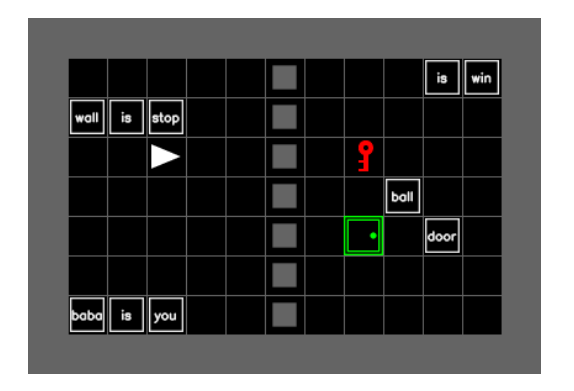
\includegraphics[width=0.5\textwidth]{iclr2025/images/babaisai_map.png} 
    \caption{One of the Baba Is AI puzzles, where the agent has to break the ``wall is stop" rule, create new rule ``door is win" and go to green door to solve the task.}
    \label{fig:babaisai_map} 
    \vspace{-2mm}
\end{figure}

\label{baba_text_wrapper}
\subsection{Baba Is AI Language Wrapper}
To enable interaction with language models, we made a custom language wrapper for Baba Is AI. It constructs language observation from active rules and creates a description by formatting object positions relative to the player. We don't provide the solution for the agent and don't specify grid boundaries in the text-only experiments.

\subsection{Baba Is AI Results}
We provide the Baba Is AI results for LLM and VLM mode in Tables \ref{babaisai_LLM} and \ref{babaisai_VLM}. Standard errors are computed using 5 seeds for each of the 40 Baba Is AI tasks. Surprisingly, the Llama models lead, with Llama 3.2 90B surpassing GPT-4o by a 10\% margin in language-only mode. Once again, when vision is added, model performance suffers, with only Gemini-1.5-Pro remaining stable.

\begin{table}[h]
    \centering
    \begin{minipage}[t]{0.48\linewidth}
    \centering
    \caption{LLM Performance on babaisai}
    \begin{tabular}{lc}
    \hline
    Model & Average Progress (\%) \\
    \hline
    llama-3.2-90b-it & 43.90 $\pm$ 3.47 \\
    llama-3.1-70b-it & 40.00 $\pm$ 3.42 \\
    claude-3.5-sonnet & 37.50 $\pm$ 4.42 \\
    gpt-4o & 33.66 $\pm$ 3.30 \\
    gemini-1.5-pro & 32.02 $\pm$ 3.26 \\
    llama-3.1-8b-it & 18.33 $\pm$ 3.53 \\
    llama-3.2-3b-it & 17.50 $\pm$ 3.47 \\
    gpt-4o-mini & 15.60 $\pm$ 2.53 \\
    llama-3.2-11b-it & 15.60 $\pm$ 2.50 \\
    gemini-1.5-flash & 12.80 $\pm$ 2.33 \\
    llama-3.2-1b-it & 10.83 $\pm$ 2.84 \\
    claude-3.5-haiku & 8.33 $\pm$ 2.52 \\
    \hline
    \label{babaisai_LLM}
    \end{tabular}
    \end{minipage}
    \hfill
    \begin{minipage}[t]{0.48\linewidth}
    \centering
    \caption{VLM Performance on babaisai}
    \begin{tabular}{lc}
    \hline
    Model & Average Progress (\%) \\
    \hline
    claude-3.5-sonnet & 34.45 $\pm$ 4.36 \\
    gemini-1.5-pro & 31.40 $\pm$ 3.24 \\
    llama-3.2-90b-it & 21.90 $\pm$ 2.89 \\
    gpt-4o & 18.62 $\pm$ 2.72 \\
    gpt-4o-mini & 16.41 $\pm$ 2.59 \\
    gemini-1.5-flash & 8.30 $\pm$ 1.92 \\
    llama-3.2-11b-it & 5.76 $\pm$ 1.63 \\
    \hline
    \label{babaisai_VLM}
    \end{tabular}
    \end{minipage}
\end{table}

\subsection{Observations}



\env{Baba Is You is a puzzle game where you can manipulate the rules of each level. 
The following are the possible actions you can take in the game, followed by a short description of each action:
\newline\newline
idle: wait for one step,\newline
up: take one step up,\newline
right: take one step to the right,\newline
down: take one step down,\newline
left: take one step to the left.\newline
\newline
Tips:\newline
- Examine the level carefully, noting all objects and text blocks present.\newline
- Identify the current rules, which are formed by text blocks in the format "[Subject] IS [Property]" (e.g. "BABA IS YOU").\newline
- Consider how you can change or create new rules by moving text blocks around.\newline
- Remember that you can only move objects or text that are not defined as "STOP" or similar immovable properties.\newline
- Your goal is usually to reach an object defined as "WIN", but this can be changed.\newline
- Think creatively about how changing rules can alter the properties and behaviors of objects in unexpected ways.\newline
- If stuck, try breaking apart existing rules or forming completely new ones.\newline
- Sometimes the solution involves making yourself a different object or changing what counts as the win condition.\newline
\newline
PLAY!
}


\env[iclr2025/images/babaisai.png]{Current Observation:\newline\newline
Active rules:\newline
baba is you\newline\newline
Objects on the map:\newline\newline
rule `is` 1 step to the left and 1 step up\newline
rule `win` 1 step up\newline
rule `key` 1 step to the left\newline
key 1 step to the right and 2 steps down\newline
ball 2 steps to the right and 3 steps down\newline
rule `baba` 2 step to the left and 4 steps down\newline
rule `is` 1 step to the left and 4 steps down\newline
rule `you` 4 steps down\newline
rule `ball` 2 steps to the right and 4 steps down\newline\newline
Image observation provided.
}

\agent{left}

